\documentclass[a4paper]{article}

\usepackage{fullpage} % Package to use full page
\usepackage{parskip} % Package to tweak paragraph skipping
\usepackage{tikz} % Package for drawing
\usepackage{amsmath}
\usepackage{hyperref}

\title{Circus Specification}
\author{Ashley J. Robinson}
\date{\today}

\begin{document}

\maketitle

\section{Introduction}

   \subsection{Acronyms} 
      \begin{table}[h]
         \centering
         \caption{Acronyms}
         \label{tab_acronyms}
         \begin{tabular}{|l|l|}
            \hline
            \textbf{Acronyms}    &  \textbf{Description}                         \\ \hline  
            ID                   &  Identity                                     \\ \hline
            IR                   &  Infra-Red                                    \\ \hline
            UART                 &  Universal Asynchronous Receiver-Transmitter  \\ \hline  
         \end{tabular}
\end{table}  


\section{Agent}

   \subsection{ID}
      \begin{itemize}
         \item Agents have hardware pin straps to configure IDs
         \item Agents have a valid ID range of 0x01 to 0xFE inclusive
         \item Agent ID = pin strap value + 1
      \end{itemize}
   
   \subsection{Receiver}
      \begin{itemize}
         \item The IR receiver will be connected to UART receiver of the microcontroller. 
      \end{itemize}


\section{Communications}
\begin{itemize}
   \item 
\end{itemize}


\begin{figure}[h]
   \centering
   \label{fig_communications}
   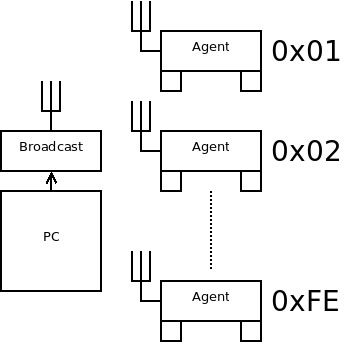
\includegraphics[width=6cm,keepaspectratio]{communications/communications.png} 
   \caption{Communication overview.}
\end{figure}

\begin{figure}[h]
   \centering
   \label{fig_communications_sm}
   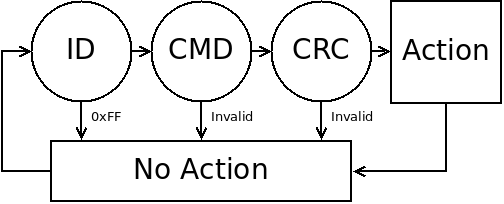
\includegraphics[width=6cm,keepaspectratio]{communications/communications_sm.png} 
   \caption{Communication state machine.}
\end{figure}


\begin{table}[h]
   \centering
   \caption{My caption}
   \label{my-label}
   \begin{tabular}{|l|l|l|l|l|l|}
        \hline
        \textbf{ID}  &  \textbf{Description} \\ \hline  
         0x00        &  Issue the following command to all agents.\\ \hline  
         0x01..0xFE  &  Issue the following command to all agents with matching IDs.\\ \hline  
         0xFF        &  Resets the agent receiver state machine. \\ \hline  
   \end{tabular}
\end{table}




\end{document}
